%%%%%%%%%%%%%%%%%%%%
\chapter{Evaluation}
% In the evaluation you convince the reader that your design works as intended.
% Describe the evaluation setup, the designed experiments, and how the experiments showcase the individual points you want to prove.
% This section is usually 5-10 pages.
%%%%%%%%%%%%%%%%%%%%
\label{chapter:evaluation}

\section{Raising Awareness with an Attack Demonstrator}

Demonstration video of the polar crane's cyberattack can be found in the \emph{NinjaCrane github}~\cite{MyGithub}. In parallel to this video a demonstration show has been created to better illustrate a real-world scenario and is detailed is the section.

\subsection{Demonstration Setup}

Two persons will act in the demonstration. The first plays the role of the polar crane's automation technician that programs the PLC with the use of his engineering workstation. The second one plays the role of the hacker. For simplicity, we assume that the hacker is in the same room as the technician. This is a violation with respect to the threat model (as a external adversary was assumed). The attacker can for example be a subcontractor. Finally the entry point used in this demonstrator is the USB Ninja cable (and not the malicious mouse).

The situation setup is the attacker talking with the technician and asking him to charge his phone (or any USB device) with the USB Ninja cable. The technician plugs the USB Ninja cable to charge his phone as shown in~\autoref{fig:plug-usb-cable}.

\begin{figure}[H]
    \centering
    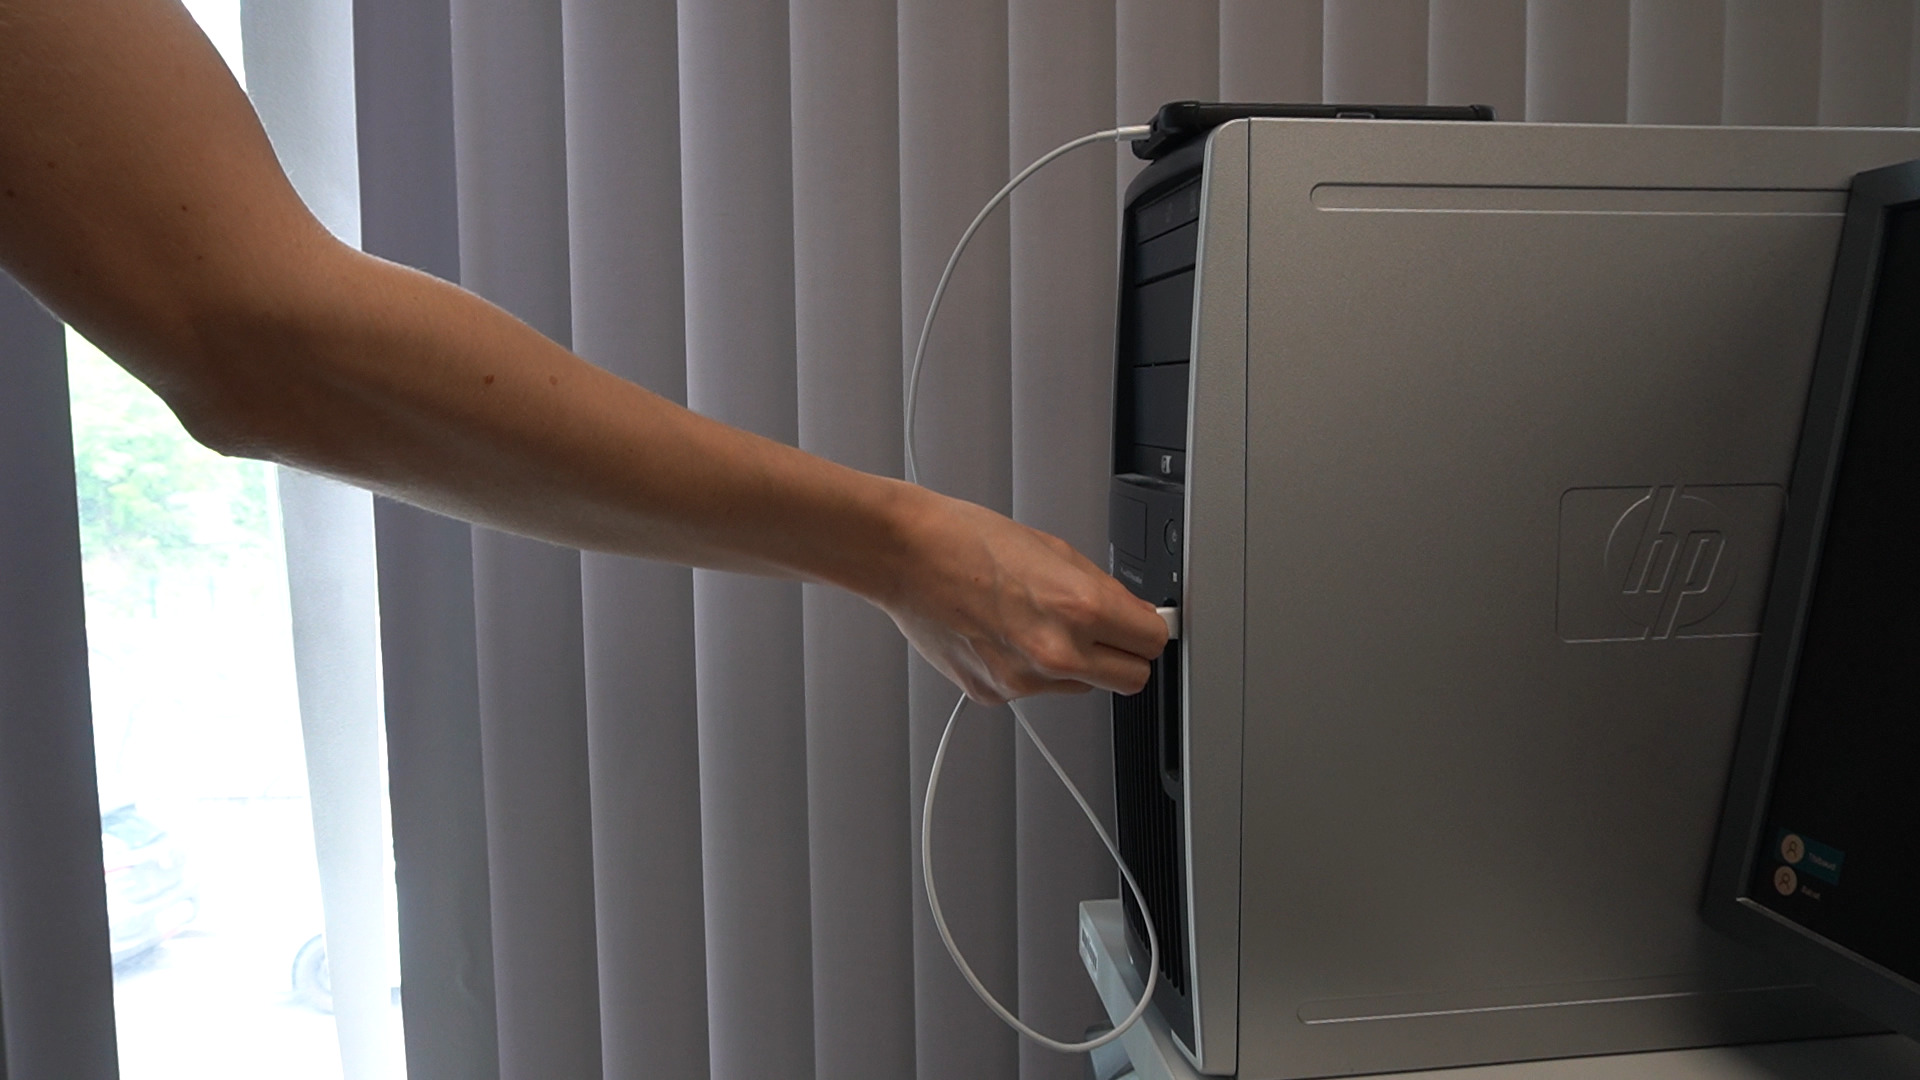
\includegraphics[trim={12cm 0 5cm 0}, clip, width=0.6\linewidth]{figures/plug-cable.jpg}
    \caption{Plugging USB Ninja Cable.}
    \label{fig:plug-usb-cable}
\end{figure}

\subsection{Engineering Workstation Infection}

Once the USB Ninja is plugged-in. The attacker will for example ask the technician to take a coffee break while leaving the session unlocked. Once done, the attacker triggers the USB Ninja cable with the adversary's GUI to run the payload. This will open the Execute service and open a powershell command in background to run the commands as shown in~\autoref{fig:execute}.

\begin{figure}[H]
    \centering
    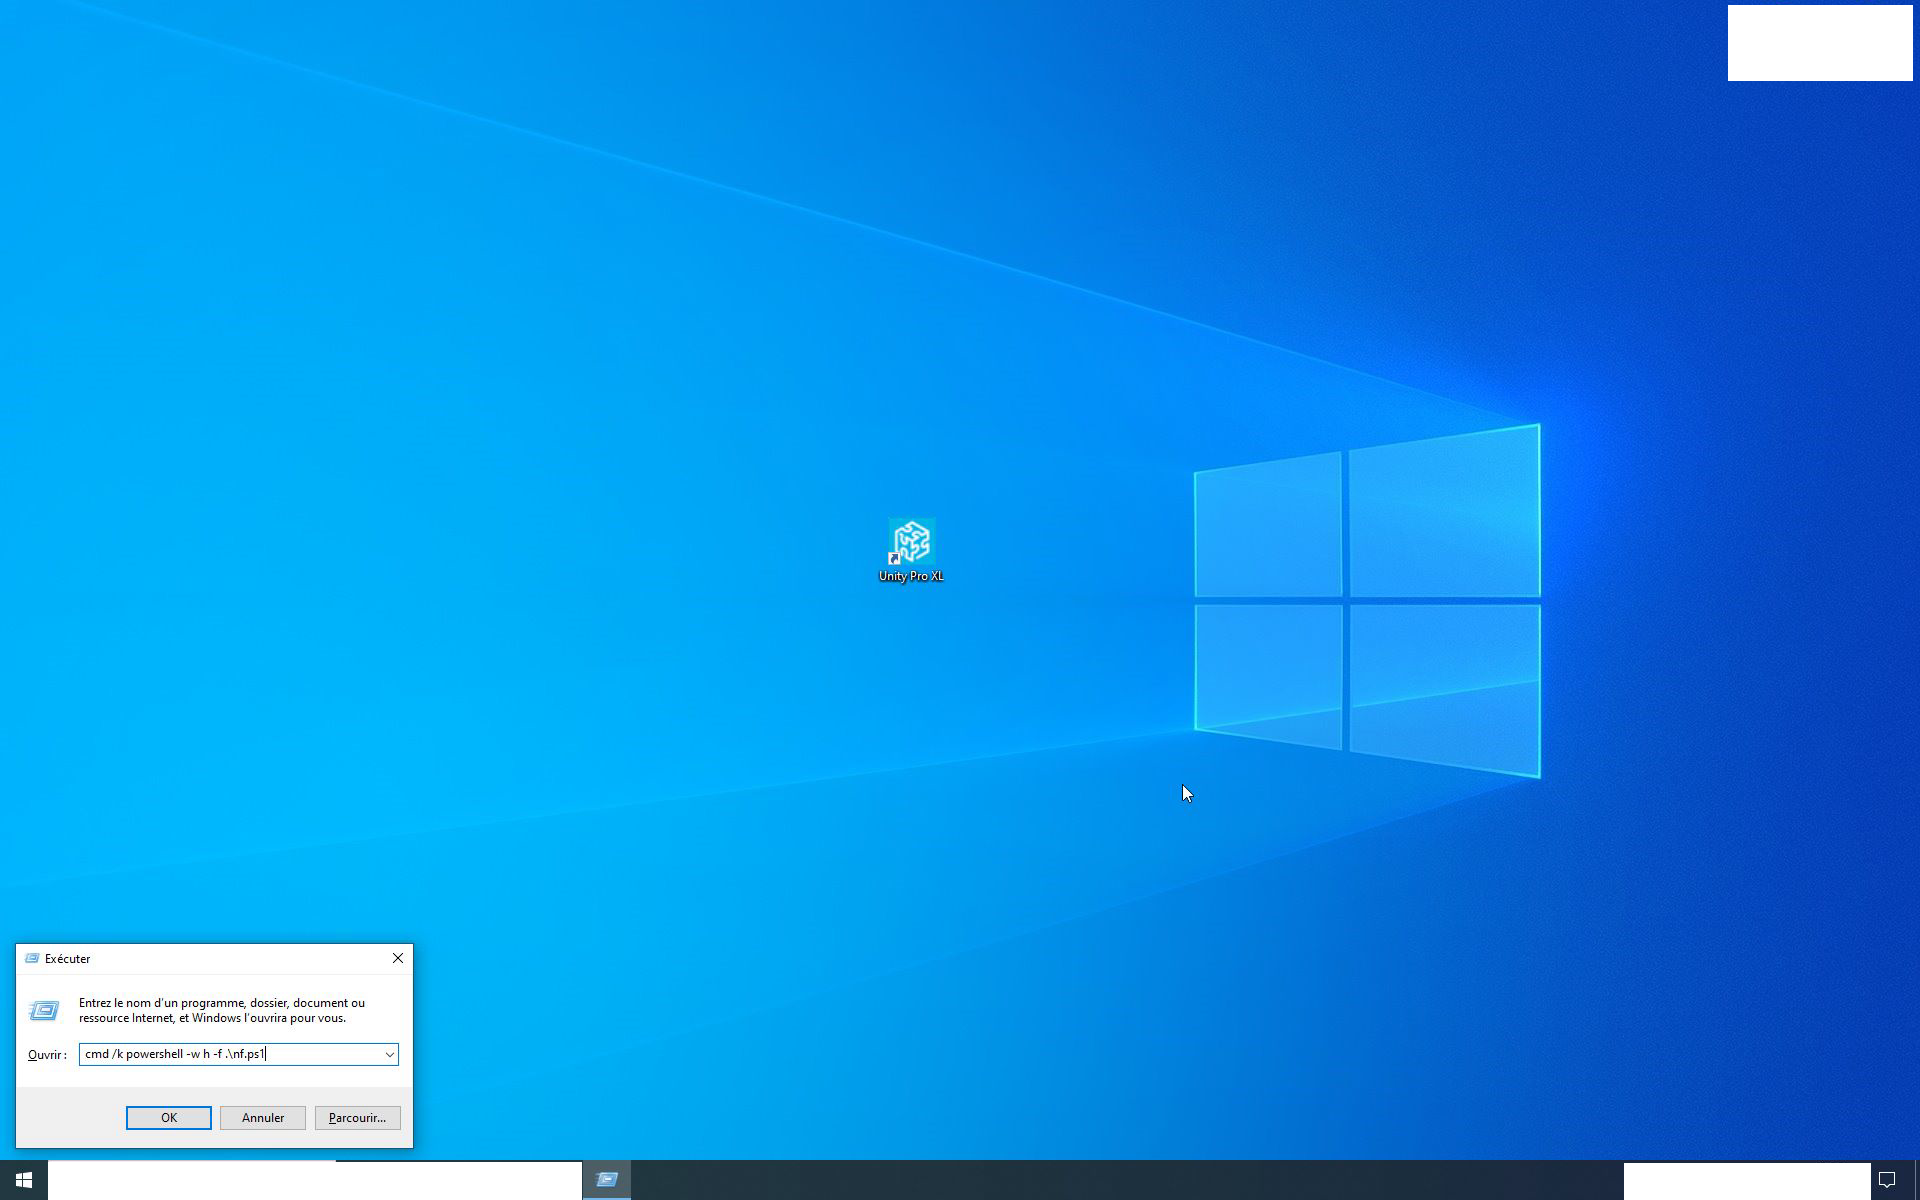
\includegraphics[trim={0cm 0cm 25cm 15cm}, clip, width=0.5\linewidth]{figures/execute.png}
    \caption{Opens the Execute service and opens a hidden powershell on the engineering workstation.}
    \label{fig:execute}
\end{figure}


The commands will create four files; \texttt{VBs.vbs} and \texttt{script.ps1} are scripts to download the malware and run it in background at each session opening, \texttt{malwar3.exe} is the downloaded \emph{NinjaCrane} malware performing the MITM attack and finally \texttt{trigger.txt} is the text file containing the instruction to triggers the polar crane's attack. The four files are created in the \texttt{Desktop/powershell\_script} folder as shown in~\autoref{fig:folder}. The~\autoref{fig:logigram} is a flowchart describing the sequence to infect to engineering workstation. For the demonstration, a modified version of the commands can be used to have an offline scenario that assumes that the \texttt{malwar3.exe} is already located at \texttt{$\backslash$Desktop$\backslash$Malware$\backslash$malwar3.exe}

\begin{figure}[H]
    \centering
    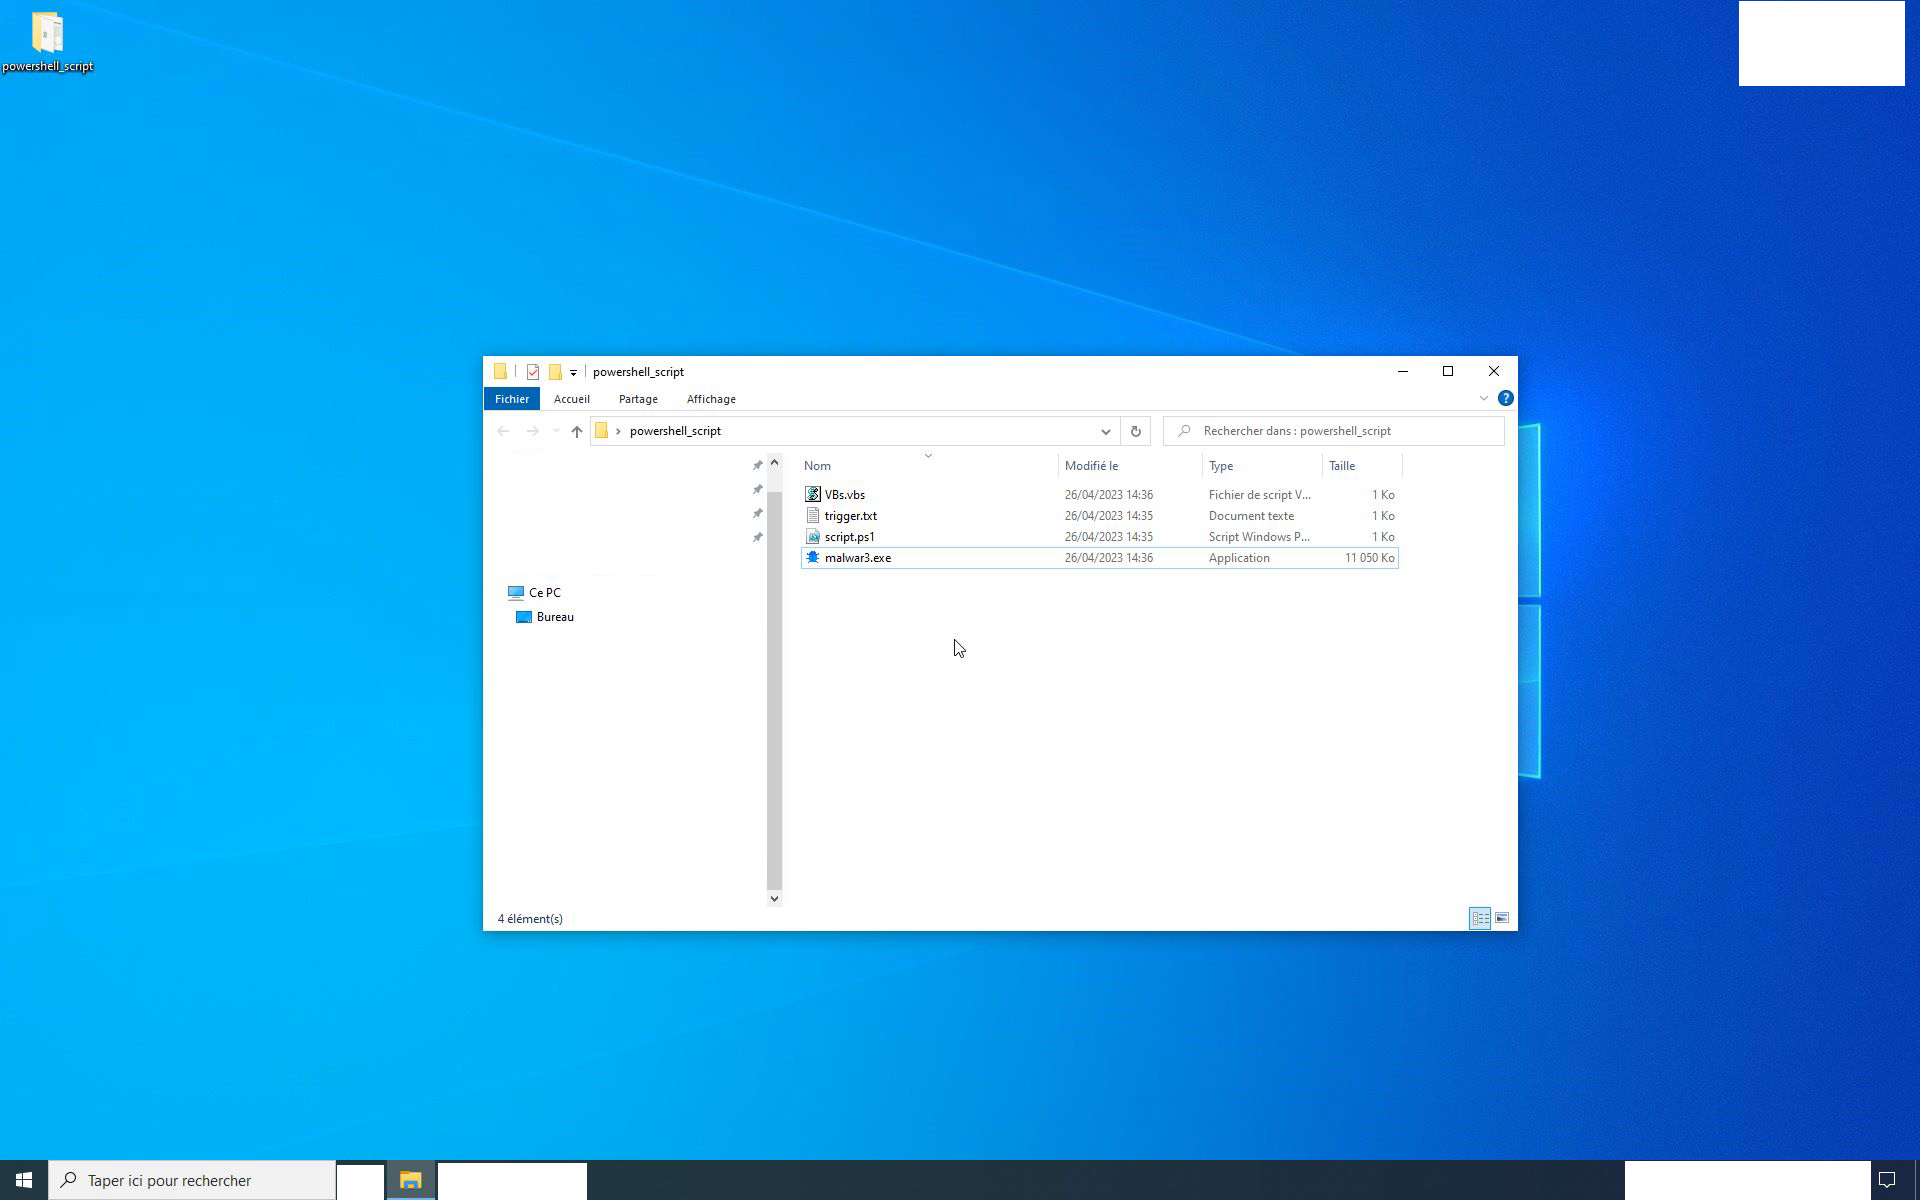
\includegraphics[trim={8cm 10cm 10cm 6cm}, clip, width=0.8\linewidth]{figures/folder.png}
    \caption{Created folders after the first USB Ninja payload execution.}
    \label{fig:folder}
\end{figure}

\subsection{Take the Polar Crane's Control}

Once the malware is running on the engineering workstation, the attacker triggers once again the USB Ninja cable to effectively disturb the polar crane as described in~\autoref{subsec:malicious-sent-packets}. The malware sends a packet to rotate the polar crane at 34\% of maximum speed then at 63\% of the maximum speed. This shows that the adversary could wear and tear the motor. Then it stops both the polar crane and the PLC. This shows that the adversary can stop the process at any time and for example stop the loaded polar crane above the reactor vessel. 

\begin{figure}[H]
    \centering
    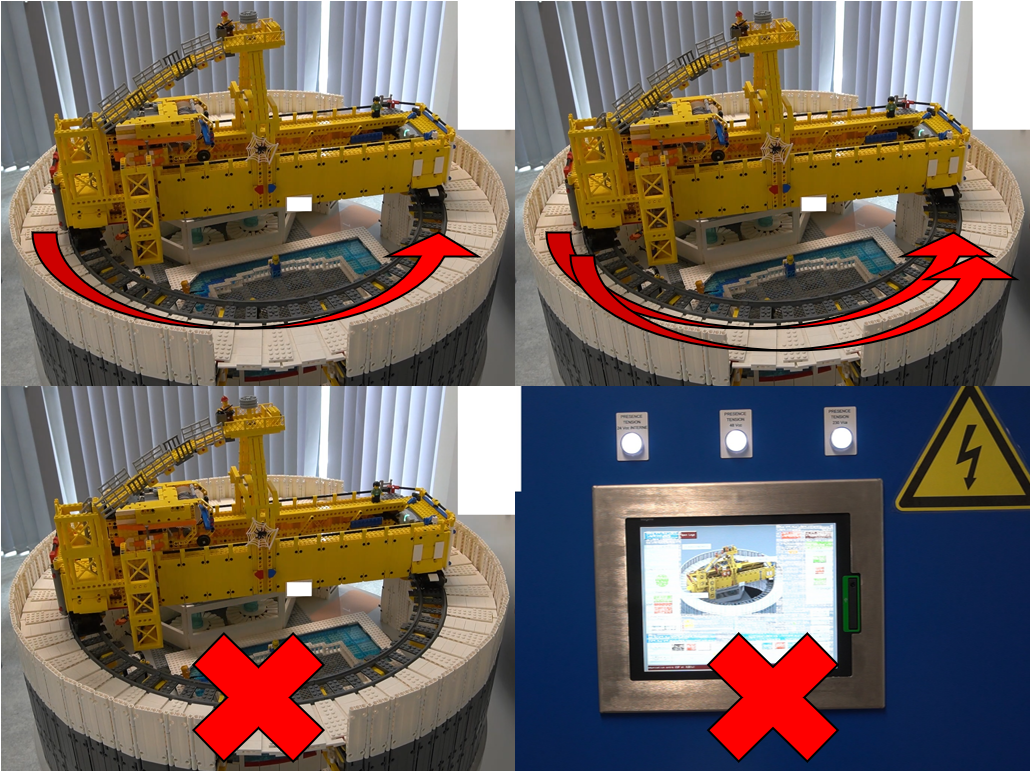
\includegraphics[width=0.9\linewidth]{figures/step-atk}
    \caption{Attack Sequence order from left to right. Top-Left: Make the polar crane rotates at 43\% of maximum speed. Top-Right: Make the polar crane rotates at higher speed (63\% of maximum speed). Bottom-Left: Stop the polar crane. Bottom-Right: Stop the PLC.}
    \label{fig:atk-steps}
\end{figure}

\section{Real World Feasibility of the Cyberattack}

\subsection{Engineering Workstation Infection}

Several observations can be made regarding the success of the engineering workstation infection.

\begin{itemize}
    \item Avast antivirus does not detect the malware executable as a threat. However, the avast antivirus fixed at a high protection level will notify the execution of the executable and ask the administrative user to block or not the execution. Moreover, the malware requires administrative privilege to execute. Thanks to the UAC bypassing method, it only requires that current logged-in user has administrative right and that the UAC level is not set to "Always Notify". 
    \item There must be no protection regarding HID-capable device. Since July 2021, the Windows environment has a built-in solution to restrict USB devices called Microsoft Intune~\cite{intune-servie},~\cite{introduce-grp-policy}. The Intune service is a system policy that blocks any USB device not matching the hardware ID whitelist given by the user.
    \item HID-based attacks come with major drawbacks. First, an event must trigger the attack. It can be a time-based event (e.g., keyboard frames are sent 10 seconds after the connection) or attacker-based event (e.g., attacker triggers the attack over BLE, as for the USB Ninja). Moreover, if windows password account is unknown to the adversary, this trigger must be run during a session unlocked. And if windows password is known to the adversary, the workstation must be turned-on. Finally, as the payload is made of keyboard frames, the attack is not completely stealth during few seconds — the time to type all the key-frames. 
\end{itemize}

\subsection{Live Demonstration Feedback}

This demonstration has been played during the \emph{Journée Sûreté} at the \emph{Direction Projet Nouveau Nucléaire }, during the \emph{Plénière} of the \emph{Département des Composants Electriques et Electromécaniques} and partially-played (i.e., only with a video support) at the \emph{Cercle d'Experts Sûrté sur la Cybersécurté} at \emph{EDF Saclay}. The demos were played with the goal to raise awareness on cybersecurity and to show how a malware could propagate from the IT to the OT systems in case of security policy breach. The demo shows a concrete social engineering scenario that leads to the industrial process failure  — the polar crane stops as well as the connection between the workstation and the PLC. Anonymously collected feedback from the demo participants can be find in~\autoref{annex:feedback}. One downside regarding the reliability of the demo can be noted. Indeed, the connection between the PLC and the engineering workstation can sometimes drop due to time-out or the engineering workstation infection must sometimes be repeated in case of bluetooth connection lost with the USB Ninja cable or if a mouse click is made during the HID-keystrokes injection.


\subsection{MITM Malware Attack}

Similarly, some observations can be made regarding the success of the MITM attack.

\begin{itemize}
    \item The MITM malware must catch the connection phase with the PLC to conduct later the attack phase. Moreover during the attack phase, engineering workstation and PLC must be connected. Unfortunately, due to connection time-out the connection between the workstation and the PLC may drop after half an hour. To overcome this, the timeout variable in Unity Pro can be increased. 
    
    \item In the current state, the \emph{NinjaCrane} attack is not resilient to program change that results in the change of variable memory location. Indeed, the attack crafts and sends pre-fixed packet to change the value of a specific memory location corresponding to a PLC's inner variable. 

    \item The attack sequence played by \emph{NinjaCrane} malware is fixed and does not consider the current state of the polar crane. During the demonstration, \emph{NinjaCrane} malware assumes that the polar crane's and PLC are already in a specific state (i.e., PLC is in run and is in the mode to control the polar crane). However, this might not be the case and the \emph{NinjaCrane} malware needs to be adjusted accordingly. For example the \emph{NinjaCrane} malware could craft some packets to read some variable states or could be made reactive by adjusting the sent packet according to the information previously gathered by observing the communication.
\end{itemize}

\section{Mitigation and Counter Measures}

\subsection{Engineering Workstation Hardening}

Solutions for engineering workstation hardening are highly-dependent on the use-case, environment, and threat model. Below is a non-exhaustive list of solutions that would have blocked the \emph{NinjaCrane} attack:

\begin{itemize}
    \item Physically blocking the USB port (e.g., Lindy USB Port Blocker). It physically prevents the use of the USB port. However the blocker can be forced and the key to unlock the blocker is any-blocker compatible.
    \item Physically blocking the data transfer wires (e.g., USB Condom). The data blocker physically prevents any data transfer but can still be used for slow charging. Charge-only cables also exist. ~\autoref{fig:data_blocker} illustrates physically how the USB data blocker works.
    \begin{figure}[H]
        \centering
        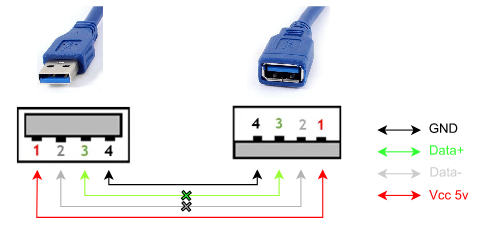
\includegraphics[height=4cm]{figures/data-blocker.png}
        \caption{Data blocker. The data blocker cuts the Data+ and Data- transmission.}
        \label{fig:data_blocker}
    \end{figure}
    \item De-activates USB port. This could be done via the BIOS, via Group Policy, Device Manager, 3rd party software, or uninstalling the USB driver.
    \item De-activates USB port based on whitelisting. This can be setup via Microsoft Intune, Group Policy or 3rd party software. USB ID device can however easily be spoofed. 
    \item \emph{USBFILTER} solution from Tian et al.~\cite{Tian15}~\cite{tian16} (or similarly \emph{Netfilter}) instruments the USB stack to filter USB packets at a fine granularity following user-defined rules. With correct rules, this solution prevents a mouse or a charging cable to act as a keyboard. Similarly the \emph{GoodUSB} solution  (currently only available for the Linux USB Stack) associate user's expectation of the device's functionality.
\end{itemize}


\subsection{Cybersecurity of the Supply Chain}

Cybersecurity over the Supply Chain is still in active development and mostly boils down to the cybersecurity principles — separation and least privilege, monitoring, life cycle development (e.g., V model), access controls, audits and regular security assessments, sensitive data encryption etc. Below is a non-exhaustive list of practical solutions that would have blocked the \emph{NinjaCrane} attack:

\begin{itemize}
    \item Blockchain technology (e.g., VeChain or ChainLink). Blockchain can help to ensure products authenticity, movements and origins via tamper-proof records available to the supply chain tenants. 
    \item In-depth inspection. Inspection can take the form of randomized security assessments of the electronic devices. By opening the maliciously tampered mouse or the USB Ninja cable the alteration would have been detected. Furthermore, characteristics inspection would also be a working lead (e.g., mouse weight or USB Ninja cable heating).
    \item Strict security policy between the tenants of the supply chain. As an example, the USB Ninja cable could be offered to an employee as a gift.
\end{itemize}
